Cette partie vise à expliquer les actions réalisées en vue de récupérer et stocker les données utilisées dans ce projet.
Au cours de cette phase plusieurs traitements permettront de réduire la quantité d'information pour se concentrer sur les corps des mails.
Les données MIME non textuelles sont écartés ainsi que les messages corrompus ou avec des encodages non convertibles en utf-8.

\subsection{Récolte des données}
	\paragraph{Recherche de dataset}
		Ma volonté initiale était de travailler sur des mails en français.
		Cependant, je n'ai pas trouvé de dataset dans cette langue.
		Je me suis donc retourné vers les dataset de mails en anglais. \\
		J'ai pu alors récupérer deux dataset :
			\begin{itemize}
				\item Enron company mails (voir~\ref{Enron_dataset})
				\item Dataset SpamAssassin (voir~\ref{SpamAssassin_dataset})
			\end{itemize}
			Les mails de SpamAssassin ont l'avantage d'être pré-trié, contrairement aux mails de la compagnie Enron.
			Ainsi le développement du moteur se fera uniquement avec les mails du SpamAssassin afin de pouvoir vérifier les résultats de l'analyse.

		\paragraph{Téléchargement des données}
			Le téléchargement du dataset Enron est possible à partir du moment où l'on possède un compte sur la plateforme Kaggle.
			Le dataset SpamAssassin est ouvert, il suffit de télécharger les archives de chaque catégorie. \\

			La récolte des données a été réalisée à la main sans automatisation.
			Les mails sont alors stockés dans plusieurs répertoires \emph{HAM} et \emph{SPAM} selon leur catégorie. \\

			Format :
			\begin{itemize}
				\item \emph{Enron} - 1 fichier CSV avec tous les mails
				\item \emph{SpamAssassin} - 1 fichier texte par mail
			\end{itemize}

	\paragraph{Evolution possible}
		La quantité de ressource disponible est assez limitée et principalement en anglais.
		Une idée aurait pu être de mettre en place un site internet où les utilisateurs peuvent fournir leurs mails avec la catégorie qu'ils estiment être la bonne. \\
		Cette solution comporte des points d'attentions.
		La confiance en l'utilisateur ne peut pas être absolue.
		Le rapport entre les ham et spam sera très probablement disproportionné en faveur des spams.
		Au vu des traitements effectués, cette solution nécessitera une gestion des données personnelles en accord avec les RGPD\@.

\subsection{Pré-traitement}
	La Figure~\ref{fig:Phase1} montre l'enchainement des étapes de traitement du mail puis du corps de texte jusqu'à la mise en base.
	Le chargement des mails en mémoire utilise le module python email (natif).
	Une grande partie des transformations sont effectuées en utilisant des expressions régulières.
	Trois points de contrôle permettent de décider si un mail sera effectivement utilisé ou non.
	\begin{enumerate}
		\item Échec de l'importation (fichier manquant lors de la tentative de lecture)
		\item Échec de récupération du corps (charset non accepté, corps vide, type du mail non textuel)
		\item Échec lors de la détermination de la langue (incapacité d'identifier les ngrams nécessaire à l'analyse)
	\end{enumerate}

	\begin{figure}[H]
		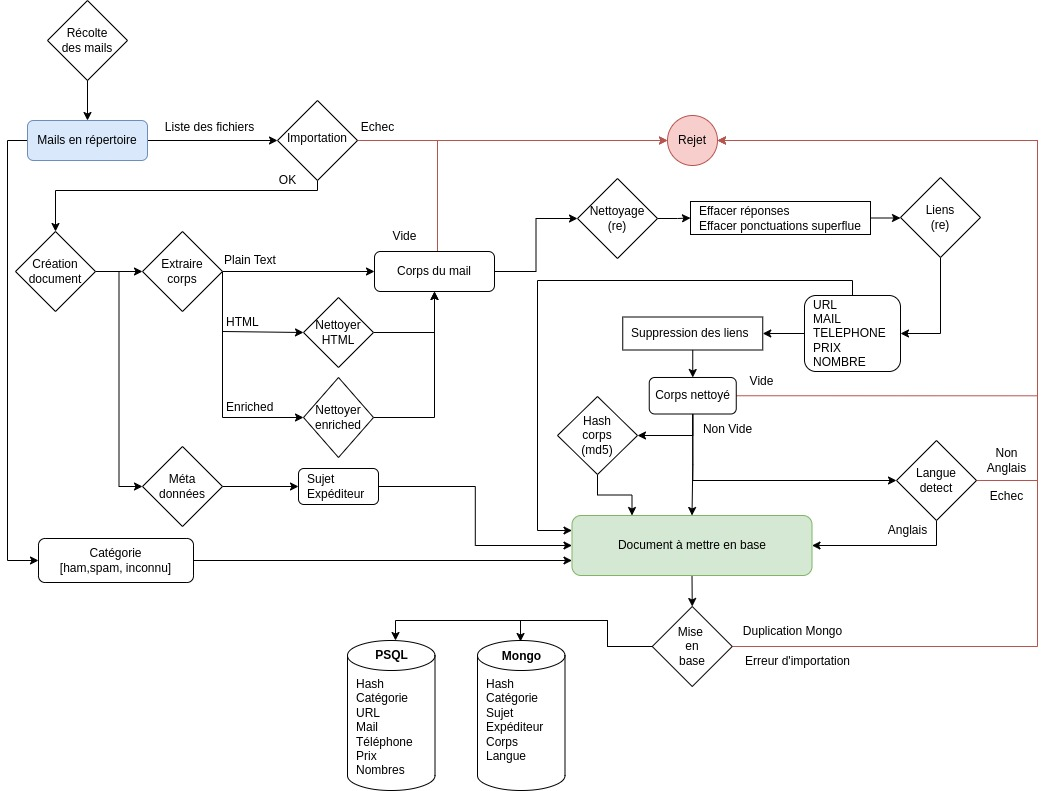
\includegraphics[width=\linewidth]{img/SchemaPhase1}
		\caption{Schéma des étapes de la phase 1}
		\label{fig:Phase1}
	\end{figure}

	\subsubsection{Importation}
		La fonction \emph{email.message\_from\_binary\_file} permet de transformer un fichier mail en objet python manipulable :
		\begin{lstlisting}[title=Fonction d'importation des fichiers,label={lst:import_file}]
def load_mail(file):
    with open(file, 'rb') as f_bin:
        return email.message_from_binary_file(f_bin)
		\end{lstlisting}

    \subsubsection{Extraction du corps des mails}
		Une fois le fichier importé au format \emph{EmailMessage}, il est possible d'en extraire le corps.
		Le corps du mail peut être composé de plusieurs parties qui ne sont pas forcément du texte.
		Les parties non textuelles ne sont pas conservée.

		\begin{lstlisting}[title=Extraction du corps du mail,label={lst:extract_corps}]
def extract_body(msg):
    refused_charset = ['unknown-8bit', 'default', 'default_charset',
                       'gb2312_charset', 'chinesebig5', 'big5']
    body = ""

    if msg.is_multipart():
        for part in msg.walk():
            if not part.is_multipart():
                body += extract_body(part)
        return body

    if msg.get_content_maintype() != 'text':
        return ""

    if msg.get_content_charset() in refused_charset:
        return ""

    if msg.get_content_subtype() == 'plain':
        payload = msg.get_payload(decode=True)
        body += payload.decode(errors='ignore')

    if msg.get_content_subtype() == 'html':
        payload = msg.get_payload(decode=True)
        body += nettoyage.clear_html(payload.decode(errors='ignore'))

    if msg.get_content_subtype() == 'enriched':
        payload = msg.get_payload(decode=True)
        body += nettoyage.clear_enriched(payload.decode(errors='ignore'))

    return body
		\end{lstlisting}

	\subsubsection{Nettoyage}
		Le nettoyage du texte utilise principalement les expressions régulières pour retirer un maximum d'éléments indésirables dans le texte.
        J'utilise également 2 modules externes afin de traiter le code HTML et faire la détection des mails qui ne sont pas écrits en anglais.

		\paragraph{Par regex}
			J'utilise le module python \emph{re} pour réaliser les traitements suivants :
			\subparagraph{Suppression des réponses}
				Lorsque l'on répond à un mail, le texte du message précédent est conservé dans le corps du mail.
                Pour permettre la distinction avec les mails précédant le caractère $>$ est ajouté en début de ligne.
                Je retire toutes les lignes correspondant à des réponses afin de limiter les doublons dans les textes.

			\begin{lstlisting}[title=Nettoyage des réponses,label={lst:clear_resp}]
def clear_reply(texte):
    pattern = re.compile('^>.*$', flags=re.MULTILINE)
    return re.sub(pattern, '', texte)
            \end{lstlisting}

			\subparagraph{Suppression des ponctuations}
				Pour ne pas surcharger la base de données et pour se concentrer sur le texte, une grande partie des caractères de ponctuation seront retirés.
                L'idée est de se concentrer sur les ponctuations classiques (.,?!).

				\begin{lstlisting}[title=Nettoyage des ponctuations,label={lst:clear_ponct}]
pattern_ponct = re.compile(r'[*#\\-_=:;<>\[\]"\'~)(|/$+}{@%&\\]', flags=re.MULTILINE)
def clear_ponctuation(texte):
    return re.sub(pattern_ponct, '', texte)
                \end{lstlisting}

			\subparagraph{Suppression des balises pour les enriched text}
				Certaines parties du corps de mail sont de type \emph{enriched text}.
				Les balises ne sont pas pertinente dans notre analyse et sont donc retirées.

				\begin{lstlisting}[title=Nettoyage des balises enriched text,label={lst:clear_enriched}]
pattern_enriched = re.compile('<.*>')
def clear_enriched(texte):
    return re.sub(pattern_enriched, '', texte)
                \end{lstlisting}

			\subparagraph{Suppression des liens}
				La présence de certaines informations comment les liens URL, les adresses mails et les numéros de téléphone ne peuvent pas être utilisés dans l'analyse textuelle.
                Cependant, il peut être intéressant de conserver une trace de leur présence.
                Nous allons ainsi modifier ces liens qui seront comptabilisés avant d'être retirés du texte.

				\begin{lstlisting}[title=Nettoyage des liens,label={lst:clear_liens}]
pattern_mail = re.compile('[a-zA-Z0-9_.+-]+@[a-zA-Z0-9-]+\\.[a-zA-Z0-9-.]+')
pattern_url1 = re.compile(r'(http|ftp|https)?://([\w\-_]+(?:(?:\.[\w\-_]+)+))'
                          r'([\w\-.,@?^=%&:/~+#]*[\w\-@?^=%&/~+#])?', flags=re.MULTILINE)
pattern_url2 = re.compile(r'(\w+\.)+\w+', flags=re.MULTILINE)
pattern_tel1 = re.compile(r'\(\d{3}\)\d+-\d+')  # (359)1234-1000
pattern_tel2 = re.compile(r'\+\d+([ .-]?\d)+')    # +34 936 00 23 23

def change_lien(texte, liens):
    temp, liens['MAIL'] = re.subn(pattern_mail, '', texte)

    temp, liens['URL'] = re.subn(pattern_url1, '', temp)
    temp, nb = re.subn(pattern_url2, '', temp)
    liens['URL'] += nb

    temp, liens['TEL'] = re.subn(pattern_tel1, '', temp)
    temp, nb = re.subn(pattern_tel2, '', temp)
    liens['TEL'] += nb

    return temp
                \end{lstlisting}

			\subparagraph{Suppression des nombres}
				Comme pour les liens, les nombres sont comptabilisés et retirés.
                Je fais la distinction entre les nombres seuls et les nombres accompagnés de sigle monétaires.
                \begin{verbatim}
                    MONNAIE = '$£€'
                \end{verbatim}
				\begin{lstlisting}[title=Nettoyage des nombres,label={lst:clear_nombre}]
pattern_prix1 = re.compile(f'[{MONNAIE}]( )?\\d+([.,]\\d+)? ', flags=re.MULTILINE)
pattern_prix2 = re.compile(f' \\d+([.,]\\d+)?( )?[{MONNAIE}]', flags=re.MULTILINE)
pattern_nb = re.compile('\\d+')

def change_nombres(texte, liens):
    temp, liens['PRIX'] = re.subn(pattern_prix1, '', texte)
    temp, nb = re.subn(pattern_prix2, '', temp)
    liens['PRIX'] += nb

    temp, liens['NOMBRE'] = re.subn(pattern_nb, '', temp)

    return temp
                \end{lstlisting}

		\paragraph{Par module}
			Lors du processus de nettoyage, j'utilise deux modules externes plus performants que ce que j'aurais pu faire simplement avec des expressions régulières.
            L'un me permet de nettoyer le code HTML, l'autre de détecter la langue du message.

			\subparagraph{Suppression du code HTML}
				Certaines parties du corps du mail sont de type HTML\@.
                J'utilise le module \emph{BeautifulSoup} pour parser le code et récupérer le texte affiché.

			    \begin{lstlisting}[title=Nettoyage des nombres,label={lst:clear_html}]
from bs4 import BeautifulSoup

def clear_html(texte):
    brut = BeautifulSoup(texte, "lxml").text
    return brut
                \end{lstlisting}
            Au cours du traitement avec ce module, j'ai eu une mise en garde.
            \begin{verbatim}
MarkupResemblesLocatorWarning - The input looks more like a filename than markup.
You may want to open this file and pass the filehandle into Beautiful Soup
            \end{verbatim}
            Après analyse, il semblerait que ce message soit levé dans le cas ou le module ne parvient pas à détecter et à récupérer le code html.
            Dans le mail concerné \\(\emph{spamassassin/spam/00307.7ed50c6d80c6e37c8cc1b132f4a19e4d}) la partie marquée comme HTML est également encodée en base64.
            \begin{verbatim}
------=_NextPart_7HZmySBWvSemNjin8Kg9YAA
Content-Type: text/html;
        charset="big5"
Content-Transfer-Encoding: base64

PGh0bWwgeG1sbnM6dj0idXJuOnNjaGVtYXMtbWljcm9zb2Z0LWNvbTp2bWwiDQp4bWxuczpvPSJ1
cm46c2NoZW1hcy1taWNyb3NvZnQtY29tOm9mZmljZTpvZmZpY2UiDQp4bWxuczp3PSJ1cm46c2No
ZW1hcy1taWNyb3NvZnQtY29tOm9mZmljZTp3b3JkIg0KeG1sbnM9Imh0dHA6Ly93d3cudzMub3Jn
L1RSL1JFQy1odG1sNDAiPg0KDQo8aGVhZD4NCjxtZXRhIGh0dHAtZXF1aXY9Q29udGVudC1UeXBl
IGNvbnRlbnQ9InRleHQvaHRtbDsgY2hhcnNldD1CaWc1Ij4NCjxtZXRhIG5hbWU9UHJvZ0lkIGNv
...         \end{verbatim}

            \subparagraph{Sélection des mails en anglais}
                Lors de mes tests, je me suis rendu compte que certains mails n'étaient pas en anglais.
                J'ai donc trouvé le module \emph{langdetect} qui permet de détecter le langage utilisé dans un texte en utilisant un modèle \emph{Naïve Bayes} avec une précision de 99\% (voir \ref{langdetect}). \\
				Je conserve dans les données à mettre en base le langage détecté avec l'idée de pouvoir traiter plusieurs langues dans le futur. \\

				La détection de la langue est réalisée juste avant la mise en base Mongo.

				\begin{lstlisting}[title=Création d'un document,label={lst:create_doc}]
import langdetect

def create_document(mail, categorie):
    corp = mail_load.extract_body(mail)
    corp, liens = nettoyage.clear_texte_init(corp)
    sujet, expediteur = mail_load.extract_meta(mail)

    if not corp:
        return None

    try:
        lang = langdetect.detect(corp)
    except langdetect.lang_detect_exception.LangDetectException:
        return None

    if lang != 'en':
        return None

    if categorie.lower() not in ['spam', 'ham']:
        categorie = 'inconnu'

    doc = {
        'hash': hashlib.md5(corp.encode()).hexdigest(),
        'categorie': categorie.lower(),
        'sujet': sujet,
        'expediteur': expediteur,
        'message': corp,
        'langue': lang,
        'liens': liens
    }
    return doc
                \end{lstlisting}


        \paragraph{Exemple de traitement}
            La section suivante montre des exemples de traitement de la phase 1.

        \begin{lstlisting}[title=Traitement initial,label={lst:clear_example_1}]
message = '''
Message dedicated to be a sample to show how the process is clearing the text.

Begin reply :
> He once said
>>> that it would be great
End of reply.

Substitutions :
spamassassin-talk@example.sourceforge.net
https://www.inphonic.com/r.asp?r=sourceforge1&refcode1=vs3390
hello.foo.bar
between $ 25 and 25,21 $

A number is : 2588,8 588
Phone type a : (359)1234-1000
Phone type b : +34 936 00 23 23
Ponctuation : ----## ..
~ ~~~~~
'''
text, liens = clear_texte_init(message)
print(liens)
print(text)
        \end{lstlisting}

        Résultat traitement initial :
        \begin{verbatim}
{'URL': 2, 'MAIL': 1, 'TEL': 2, 'NOMBRE': 3, 'PRIX': 2}

Message dedicated to be a sample to show how the process is clearing the text.

Begin reply


End of reply.

Substitutions



between and

A number is  ,
Phone type a
Phone type b
Ponctuation   ..
        \end{verbatim}

        \begin{lstlisting}[title=Traitement HTML,label={lst:clear_example_html}]
message_html = '''
<!DOCTYPE html PUBLIC "-//W3C//DTD HTML 4.01 Transitional//EN">
<html>
<head>
  <title>Foobar</title>
</head>
<body>
I actually thought of this kind of active chat at AOL
bringing up ads based on what was being discussed and
other features
  <pre wrap="">On 10/2/02 12:00 PM, "Mr. FoRK"
  <a class="moz-txt-link-rfc2396E"href="mailto:fork_
  list@hotmail.com">&lt;fork_list@hotmail.com&gt;</a>
  wrote: Hello There, General Kenobi !?
<br>
</body>
</html>
'''
print(clear_html(message_html))
        \end{lstlisting}
        Résultat traitement HTML :
        \begin{verbatim}

Foobar


I actually thought of this kind of active chat at AOL
bringing up ads based on what was being discussed and
other features
  On 10/2/02 12:00 PM, "Mr. FoRK"
  <fork_list@hotmail.com>
  wrote: Hello There, General Kenobi !?


        \end{verbatim}

        \begin{lstlisting}[title=Traitement enriched text,label={lst:clear_example_enriched}]
message_enriched = '''
<smaller>I'd like to swap with someone also using Simple DNS to take
advantage of the trusted zone file transfer option.</smaller>
'''
print(clear_enriched(message_enriched))
        \end{lstlisting}

        Résultat traitement enriched text :
        \begin{verbatim}
I'd like to swap with someone also using Simple DNS to take
advantage of the trusted zone file transfer option.
        \end{verbatim}


\subsection{Mise en base}
    La mise en base et le dernier traitement de cette phase.
    Les traitements précédents ont créé une liste de dictionnaires python contenant les valeurs à sauvegarder (document).
    Chaque document répond au schéma défini dans le tableau~\ref{tab:mapping_fouille} \\
    \begin{table}[H]
        \centering
        \begin{tabular}{lccr}
            Clé & Mongo & PSQL & Description\\
            \hline
            hash & \_id & messages(hash) & signature md5 du corp\\
            categorie & categorie & categories(nom) & ham, spam, inconnu\\
            sujet & sujet & & sujet du mail\\
            expediteur & expediteur & & source du mail\\
            message & message & & corps du mail\\
            langue & langue & & en\\
            liens['URL'] & & liens(url) & nombre d'url\\
            liens['MAIL'] & & liens(mail) & nombre d'adresses mail\\
            liens['TEL'] & & liens(tel) & nombre de numéros de téléphone\\
            liens['PRIX'] & & liens(prix) & nombre de références à des prix\\
            liens['NOMBRE'] & & liens(nombre) & nombre d'apparitions de nombres\\
            \hline
        \end{tabular}
        \caption{Mapping des clés python avec les bases de données}
        \label{tab:mapping_fouille}
    \end{table}

    La valeur du hash va permettre d'exclure les doublons qui ont déjà été insérés dans les bases MongoDB et PSQL\@.
    Cette valeur va également permettre de faire la liaison entre les données des différentes bases.\\
    Le schéma~\ref{fig:BddPhase1} illustre l'état des relations entre les bases de données PSQL et Mongo.

    \begin{figure}[H]
		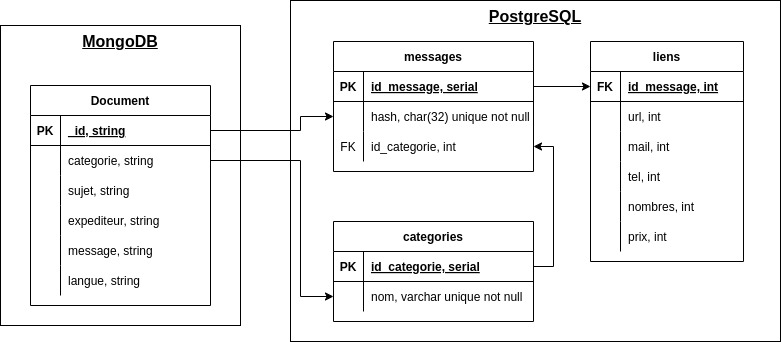
\includegraphics[width=\linewidth]{img/bddFouille}
		\caption{Relation entre les bases de données}
		\label{fig:BddPhase1}
	\end{figure}

    \paragraph{Wrapper en python}
        La communication entre le programme et les bases de données se fait au moyen des modules suivants :
        \begin{itemize}
            \item[-] MongoDB - pymongo (bibliothèque officielle maintenue par mongoDB)
            \item[-] PSQL - psycopg2 (bibliothèque open-source), utilisée pour les requêtes simples
            \item[-] PSQL - sqlalchemy (bibliothèque open-source), utilisée pour les requêtes complexes
            \item[-] SQLite - sqlite3 (bibliothèque standard de python)
        \end{itemize}

        Des modules internes au programme ont été développer pour simplifier l'utilisation des modules d'interaction avec les bases de données.
        Les packages cmd\_mongo.py, cmd\_psql.py, cmd\_sqlite.py regroupent les fonctions qui sont utilisées pour les intéractions entre le programme et les bases respectives.

    \paragraph{Problèmes éventuels}
        Lors de l'insertion les cas suivants sont susceptibles d'arriver si les deux bases n'ont pas été correctement nettoyées.\\
        \begin{table}[H]
            \centering
            \begin{tabular}{|p{4cm}|p{4cm}|p{7cm}|}
                \hline
                Situation & Raison & Solution\\
                \hline
                Mail présent dans Mongo et absent dans PSQL & Échec d'insertion dans la base PSQL & Supprimer l'entrée dans la base Mongo et relancer le traitement pour ce mail\\
                \hline
                Mail présent dans PSQL et absent dans Mongo & Suppression du mail dans la base Mongo & Supprimer le mail et toutes ses références dans la base PSQL et relancer le traitement de ce mail\\
                \hline
            \end{tabular}
            \caption{Problèmes possibles avec la mise en base}
            \label{tab:pb-base}
        \end{table}


    \paragraph{Stockage des données statistiques du traitement - SQLite}
        Les données présentent dans cette base permettent de suivre l'évolution de certaines métriques lors des différentes étapes du nettoyage.
        Lors de chaque étape de la phase 1 (Récolte, Création des documents, Mise en base), je calcule pour les HAM, SPAM et (HAM+SPAM) les éléments suivants :
        \begin{itemize}
            \item[-] mails - nombre de mails
            \item[-] mots - nombre de mots dans tout le corpus
            \item[-] mots\_uniques - nombre de mots uniques dans tout le corpus
        \end{itemize}

        Ces données me permettent d'estimer la quantité de données nettoyées durant cette phase.

        \begin{figure}[H]
            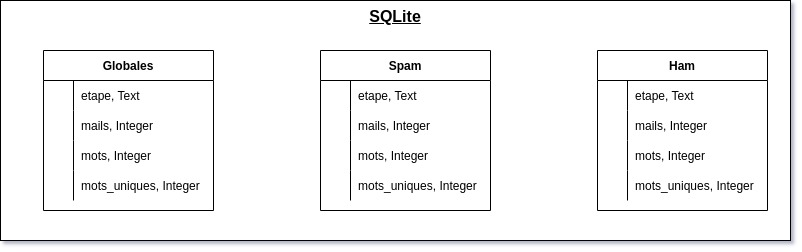
\includegraphics[width=\linewidth]{img/Schemasqlite}
            \caption{Schéma de la base de données pour lors du traitement}
            \label{fig:sqlite_schema}
        \end{figure}

\subsection*{Analyse}
    L'exécution du programme donne les informations présentées dans le tableau~\ref{tab:fouillestats}.
    \begin{table}
\caption{Données statistiques de la fouille}
\label{tab:fouillestats}
\begin{tabular}{l|rrr|rrr|rrr}
\toprule
 & \multicolumn{3}{c}{mails} & \multicolumn{3}{c}{mots} & \multicolumn{3}{c}{mots\_uniques} \\
categorie & globales & spam & ham & globales & spam & ham & globales & spam & ham \\
etape &  &  &  &  &  &  &  &  &  \\
\midrule
récolte & 5798 & 1897 & 3901 & 2385120 & 916756 & 1468364 & 262614 & 129090 & 133524 \\
création & 5658 & 1784 & 3874 & 1222793 & 589119 & 633674 & 99772 & 40615 & 59157 \\
mise\_en\_base & 5333 & 1528 & 3805 & 1163550 & 533441 & 630109 & 99772 & 40615 & 59157 \\
\bottomrule
\end{tabular}
\end{table}

    
    La figure~\ref{fig:dashFouille} montre un aperçu des données statistiques récoltées durant cette première phase.
    Les 3 premiers graphiques montrent l'évolution du nombre de documents, de mots et de mots uniques en fonction des étapes intermédiaires.\\
    Cette visualisation permet de faire les observations suivantes :
    \begin{itemize}
        \item[-] La diminution des documents spam est plus importante que celle des ham
		\item[-] Le nombre de mots uniques ne diminue plus après la création de document
		\item[-] La diminution du nombre de mots est plus importante dans les ham que dans les spam
		\item[-] Le nombre de mots uniques est plus important dans les ham que dans les spam
    \end{itemize}
    Après la phase de récolte, on remarque qu'il y a un nombre plus important de document en double dans la catégorie \emph{spam}.
    Il y a également une réduction importante du nombre de mots ainsi que du nombre de mots uniques dans les \emph{ham}.
    Cette réduction peut s'expliquer par le nettoyage du corps des mails :
    \begin{itemize}
        \item Retrait des réponses
        \item Retrait de certaines ponctuations
        \item Suppression des balises HTML et enriched text
        \item Retrait des liens, et nombres
    \end{itemize}

    Enfin, on peut voir que les \emph{ham} utilisent plus de mots uniques que les \emph{spam}.
    Il est donc possible que le vocabulaire des \emph{spam} soit plus restreint.
    \begin{figure}[H]
        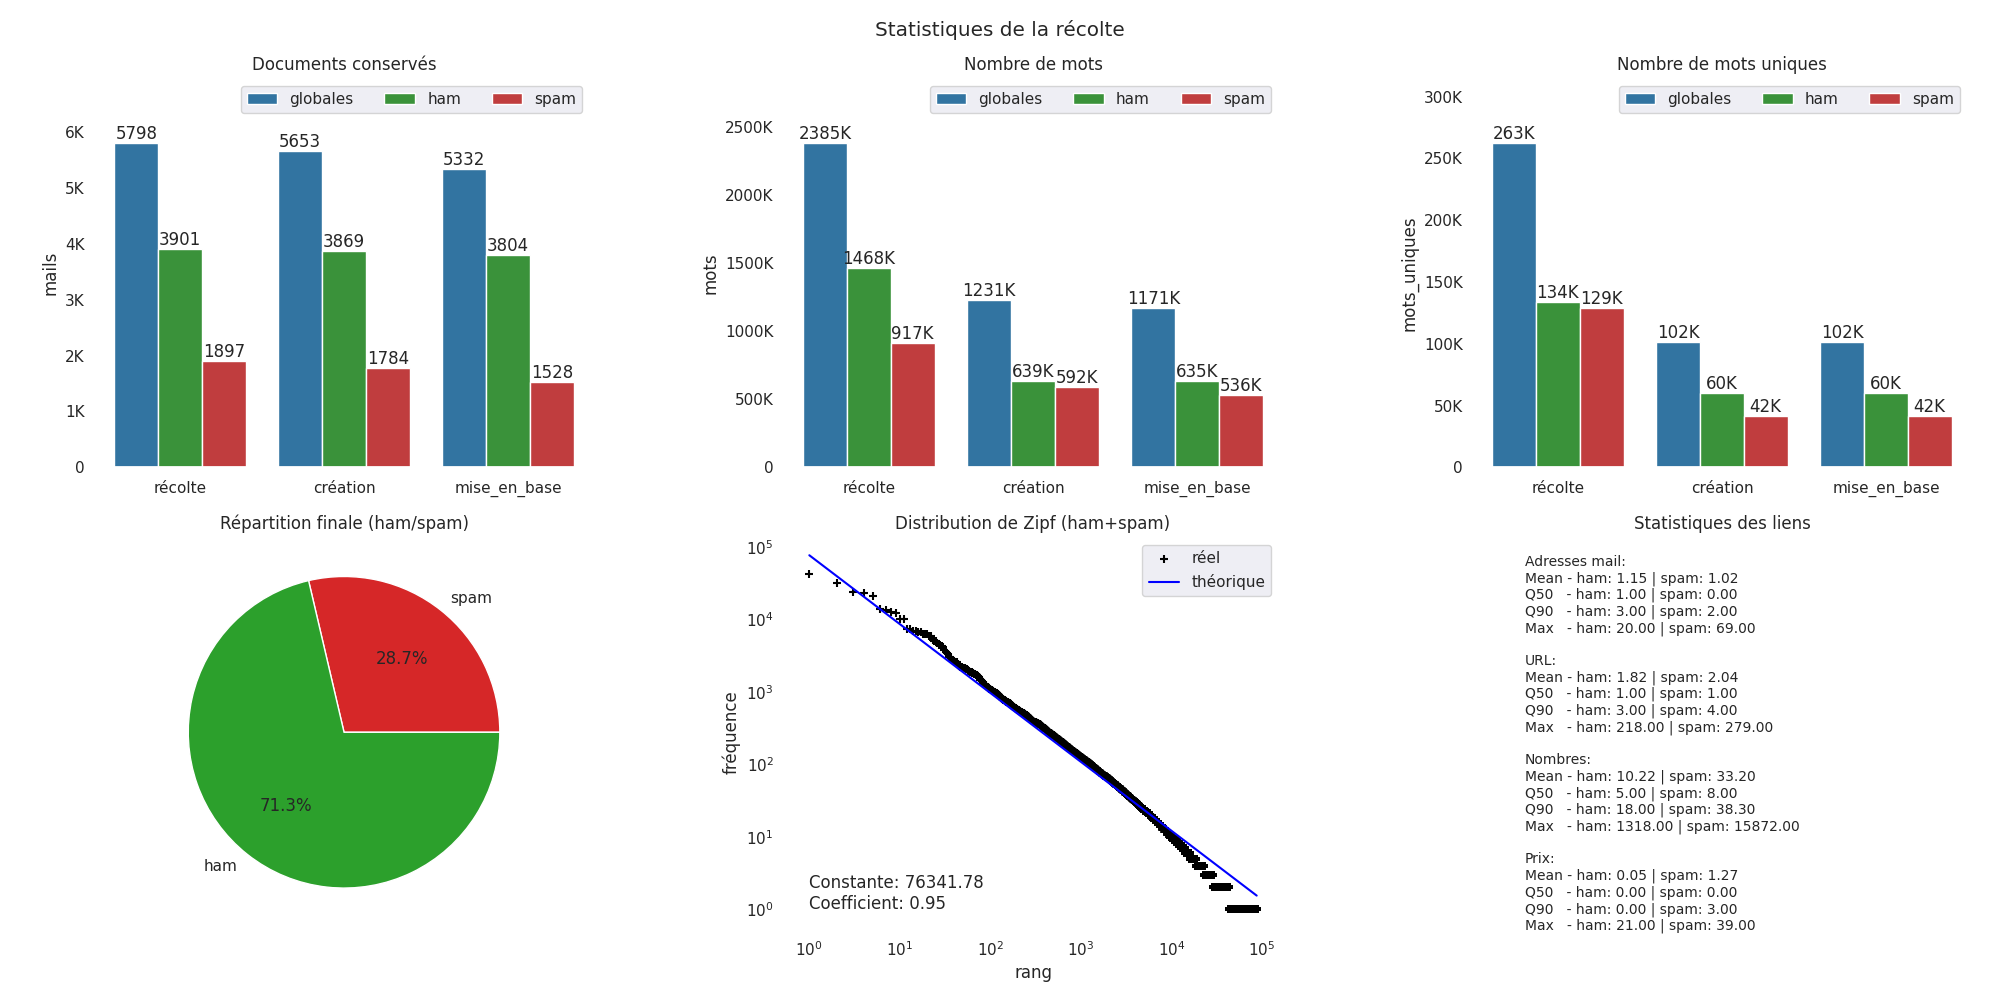
\includegraphics[width=\linewidth]{img/fouilleStats}
        \caption{Tableau de bord de la fouille}
        \label{fig:dashFouille}
    \end{figure}

    À l'issue de ces traitements, la proportion dans notre dataset ham/spam est d'environ 70/30.
    On voit aussi que la distribution du Zipf est globalement respectée.
    Il est ainsi fortement probable que notre dataset respecte les caractéristiques linguistiques naturelles.\\

    L'extraction des liens et des informations numériques donne les statistiques du tableau~\ref{tab:p1liens}.
%    \begin{table}[H]
%        \centering
%        \begin{tabular}{l|rr|rr|rr|rr|rr}
%            & \multicolumn{2}{c}{url} & \multicolumn{2}{c}{mail} & \multicolumn{2}{c}{tel} & \multicolumn{2}{c}{prix} & \multicolumn{2}{c}{nombre}\\
%            & spam & ham & spam & ham & spam & ham & spam & ham & spam & ham\\
%            \hline
%            moyenne & 5.25 & 3.83 & 1.01 & 1.13 & 0.06 & 0.20 & 0.81 & 0.03 & 30.36 & 7.1\\
%            médiane & 3 & 2 & 0 & 1 & 0 & 0 & 0 & 0 & 7 & 4\\
%            90\% & 9 & 6 & 2 & 3 & 0 & 1 & 2 & 0 & 35 & 14\\
%            maximum & 295 & 470 & 69 & 20 & 67 & 25 & 29 & 17 & 15801 & 731\\
%        \end{tabular}
%        \caption{Statistiques sur les liens et informations numériques}
%        \label{tab:p1lien_old}
%    \end{table}
    Les données statistiques sur les liens ne permettent pas mettre en avant une différence franche dans l'utilisation de ces éléments dans les catégories observées.
    Seul la présence de nombres ou d'URL seraient éventuellement susceptible d'apporter une aide à la catégorisation.
    \begin{table}[H]
\centering
\caption{Statistiques sur les liens et informations numériques}
\label{tab:p1liens}
\begin{tabular}{ll|rrr}
\toprule
 & categorie & ham & spam \\
\midrule
\multirow[c]{4}{*}{url} & mean & 3.81 & 5.26 \\
 & q50 & 2.0 & 3.0 \\
 & q90 & 6.0 & 9.0 \\
 & max & 470.0 & 295.0 \\
\cline{1-4}
\multirow[c]{4}{*}{mail} & mean & 1.15 & 1.02 \\
 & q50 & 1.0 & 0.0 \\
 & q90 & 3.0 & 2.0 \\
 & max & 20.0 & 69.0 \\
\cline{1-4}
\multirow[c]{4}{*}{tel} & mean & 0.21 & 0.06 \\
 & q50 & 0.0 & 0.0 \\
 & q90 & 1.0 & 0.0 \\
 & max & 25.0 & 67.0 \\
\cline{1-4}
\multirow[c]{4}{*}{nombre} & mean & 7.16 & 30.35 \\
 & q50 & 4.0 & 7.0 \\
 & q90 & 14.0 & 34.3 \\
 & max & 731.0 & 15801.0 \\
\cline{1-4}
\multirow[c]{4}{*}{prix} & mean & 0.04 & 0.81 \\
 & q50 & 0.0 & 0.0 \\
 & q90 & 0.0 & 2.0 \\
 & max & 17.0 & 29.0 \\
\cline{1-4}
\bottomrule
\end{tabular}
\end{table}


\subsection*{Choix techniques}
    \paragraph{Langage de programmation}
        Python a été choisi pour développer ce programme pour les raisons énoncées ci-dessous :
        \begin{itemize}
            \item[-] Large choix de modules, dont plusieurs spécialisés dans le traitement de données
            \item[-] Langage simple et flexible
            \item[-] Facilement portable et executable avec la fourniture des environnements virtuel
        \end{itemize}

    \paragraph{Métriques}
        L'utilisation du nombre de documents, de mots et de mots uniques pour mesurer la performance de cette phase a été commandée par le cours.
        Il n'y a pas eu de difficultés majeures sur cette partie.
        Ces données ne sont pas conservées au fur et à mesure des diverses importations.
        Je n'ai pas jugé pertinent de les employer lors des traitements futurs. \\

        La recherche des apparitions d'adresse mail, de liens url, de numéros de téléphone, de prix et de nombres est une idée personnelle.
        Je voulais voir si ces éléments étaient susceptible d'être discriminant pour la classification.
        Les résultats ne sont pas aussi marqués que je ne l'aurais cru.
        Je pense qu'il aurait été possible d'améliorer la justesse de ces données en travaillant sur plus de cas possible.
        Ou en analysant plus en profondeur les substitutions effectuées notamment sur les nombres.\\
        Cela étant la substitution et effacement de ces éléments dans le corps de texte peut répondre à une nécessité d'anonymisation.
        De plus la suppression des liens URL évite de conserver et de rendre accessible des liens potentiellement frauduleux.\\

        Le développement du code pour la distribution de ZIPF a été réalisée suite à une discussion avec le professeur.
        Initialement, je souhaitais également tester cette distribution sur chaque message individuellement.
        Mais la quantité de mots par message n'est peut-être pas suffisant pour obtenir des résultats probants.
        J'ai dû me renseigner beaucoup pour arriver à comprendre l'équation sous-jacente et comment je pouvais la coder de manière efficace et visuelle.
        Vous pouvez voir le résultat de ce travail dans l'annexe~\ref{sec:devZipf}.

\newpage
\subsection*{Exemple de commandes pour exécuter la fouille}
    \begin{verbatimtab}
$ make venv
$ make docker_start
cd ./src/infra/; docker compose up -d; cd -
[+] Running 3/3
 ✔ Network infra_default    Created                                                                                                                                                                           0.1s
 ✔ Container infra-mongo-1  Started                                                                                                                                                                           0.5s
 ✔ Container infra-pgdb-1   Started

$ source .venv/bin/activate
(.venv)$ ./errol.py fouille -g \
        -a ./project_data/spamassassin/easy_ham \
           ./project_data/spamassassin/easy_ham_2 \
        -p ./project_data/spamassassin/spam \
           ./project_data/spamassassin/spam_2
    \end{verbatimtab}

    Il est possible d'accéder aux bases de données avec les commandes suivantes:
    \begin{verbatimtab}
$ sqlite3 project_database/sqlite/metrics.db
$ psql -h localhost -p 5432 errol psql_errol
$ mongosh -u mongo_errol -p <MOT DE PASSE> errol
    \end{verbatimtab}